% -------------------------------------------------------------------------------
% Establish page structure & font.
\documentclass[12pt]{report}

\usepackage[total={6.5in, 9in},
	left=1in,
	right=1in,
	top=1in,
	bottom=1in,]{geometry} % Page structure

\usepackage{graphicx} % Required for inserting images
\graphicspath{{../.images/}} % Any additional images I use (BCU logo, etc) are from here.

\usepackage[utf8]{inputenc} % UTF-8 encoding
\usepackage[T1]{fontenc} % T1 font
\usepackage{float}  % Allows for floats to be positioned using [H], which correctly
                    % positions them relative to their location within my LaTeX code.
\usepackage{subcaption}

\usepackage{pdflscape} % Enables the page to be rotated 
                       % landscape for easier image viewing.

% -------------------------------------------------------------------------------
% Declare biblatex with custom Harvard BCU styling for referencing.
\usepackage[
    useprefix=true,
    maxcitenames=3,
    maxbibnames=99,
    style=authoryear,
    dashed=false, 
    natbib=true,
    url=false,
    backend=biber
]{biblatex}

% Additional styling options to ensure Harvard referencing format.
\renewbibmacro*{volume+number+eid}{
    \printfield{volume}
    \setunit*{\addnbspace}
    \printfield{number}
    \setunit{\addcomma\space}
    \printfield{eid}}
\DeclareFieldFormat[article]{number}{\mkbibparens{#1}}

% Declare it as the bibliography source, to be called later via \printbibliography
\addbibresource{litReview.bib}

% -------------------------------------------------------------------------------
% To prevent "Chapter N" display for each chapter
\usepackage[compact]{titlesec}
\usepackage{wasysym}
\usepackage{import}

\titlespacing*{\chapter}{0pt}{-2cm}{0.5cm}
\titleformat{\chapter}[display]
{\normalfont\bfseries}{}{0pt}{\Huge}

% -------------------------------------------------------------------------------
% Custom macro to make an un-numbered footnote.

\newcommand\blfootnote[1]{
    \begingroup
    \renewcommand\thefootnote{}\footnote{#1}
    \addtocounter{footnote}{-1}
    \endgroup
}

% -------------------------------------------------------------------------------
% Fancy headers; used to show my name, BCU logo and current chapter for the page.
\usepackage{fancyhdr}
\usepackage{calc}
\pagestyle{fancy}

\setlength\headheight{37pt} % Set custom header height to fit the image.

\renewcommand{\chaptermark}[1]{%
    \markboth{#1}{}} % Include chapter name.


% Lewis Higgins - ID 22133848           [BCU LOGO]                [CHAPTER NAME]
\lhead{Lewis Higgins - ID 22133848~~~~~~~~~~~~~~~
\includegraphics[width=1.75cm]{BCU}}
\fancyhead[R]{\leftmark}

% ------------------------------------------------------------------------------
% Used to add PDF hyperlinks for figures and the contents page.

\usepackage{hyperref}

\hypersetup{
    colorlinks=true,
    linkcolor=black,
    filecolor=magenta,
    urlcolor=blue,
    citecolor=black,
}

% ------------------------------------------------------------------------------
\usepackage{xcolor} 
\usepackage{colortbl}
\usepackage{longtable}
\usepackage{amssymb}
% ------------------------------------------------------------------------------

% ------------------REMOVE ME --------------------------------------------------

% Temp, using to add notes for the draft edition.
\usepackage{tcolorbox}

% ----------------- REMOVE ME --------------------------------------------------

\begin{document}

    \makeatletter
    \begin{titlepage}
        
\includegraphics[width=0.3\linewidth]{BCUWide.jpg}\\[4ex]
        \vspace{1cm}
        \begin{center}
            {\huge \bfseries  CMP6200}\\[2ex]
            {\huge \bfseries  Individual Undergraduate Project}\\[2ex]
            {\huge \bfseries 2024 - 2025}\\[6ex]
            {\large \bfseries A2 - Literature Review and Methods}\\[10ex]
            {\huge \bfseries University Artifically Intelligent Assistant}\\[6ex]
            
\includegraphics[width=0.1\linewidth]{Symbol.png}\\[40ex]
            Course: Computer \& Data Science\\
            Student Name: Lewis Higgins\\
            Student Number: 22133848\\
            Supervisor Name: Dr. Atif Azad
        \end{center}
    \end{titlepage}
    \makeatother
    \thispagestyle{empty}
    \newpage

    \tableofcontents
    %\footnotesize{\listoffigures}

    \chapter{Report Introduction}\label{ch:introduction}

    \begin{tcolorbox}[colback=orange!5!white,colframe=orange!75!black,title=Draft notice]
        This is a very early draft of this literature review and will be subject to major change
        over the next month. I've marked sections that I've taken from the proposal, or ones that 
        I'm currently uncertain of, with boxes similar to this one.
    \end{tcolorbox}


    \section{Aims and Objectives}

    \begin{tcolorbox}[colback=red!5!white,colframe=red!75!black,title=Copied from proposal]
        These are still subject to change pending the feedback from my proposal.
    \end{tcolorbox}

    This project aims to aid new and existing students alike while they are attending university with 
    helpful information about the university itself, such as university societies, locations/campuses, 
    and policies through the medium of a digital chatbot companion to converse with.
    Its objectives are to:

    \begin{itemize}
        \item Develop a chatbot capable of accurately answering user queries related to university 
        buildings, policies, and societies with a minimum 95\% accuracy rate.
        \item Conduct a thorough literature review on the surrounding topics, namely AI, LLMs and NLP.
        \item Create effective documentation for all stages of development, highlighting challenges faced during the process.
        \item Manage time effectively to ensure all project milestones are met on a consistent and regular timeframe.
        \item Evaluate the effectiveness of an AI assistant on university student acclimatization.
    \end{itemize}

    \pagebreak % REMOVE ME IF UNNECESSARY

    \section{Literature Search Methodology}

    \begin{tcolorbox}[colback=yellow!5!white,colframe=yellow!75!black,title=Uncertainty - Unfinished section]
        I assumed that I should include the exact search terms including special characters
        like asterisks as well as AND + OR queries, but I'm not sure how to best display that
        in this document. I'm also aware that a few of these are parts of each other (Deep learning
        and NLP for example) though I would surely need to research both anyway?
    \end{tcolorbox}

    \noindent 
    My literature search will be performed using multiple reputable databases for academic papers, including:
    \begin{itemize}
        \item IEEE Xplore
        \item Scopus / Elsevier
        \item Google Scholar
        \item BCU Online Library
    \end{itemize}
    
    \noindent By using multiple different databases to source my information from, I can ensure that
    any potentially relevant literature will be found. Figure \ref{fig:litSearch} depicts 
    how in a search for 1685 articles about employee retention strategies and turnover, only 582 (25.7\%) appeared in multiple databases
    \autocite{litSearch}, meaning that the remaining 74.3\% of articles were exclusive to the single 
    database in which they were found, emphasising the importance of searching multiple databases.  

    \begin{figure}[H]
        \centering
        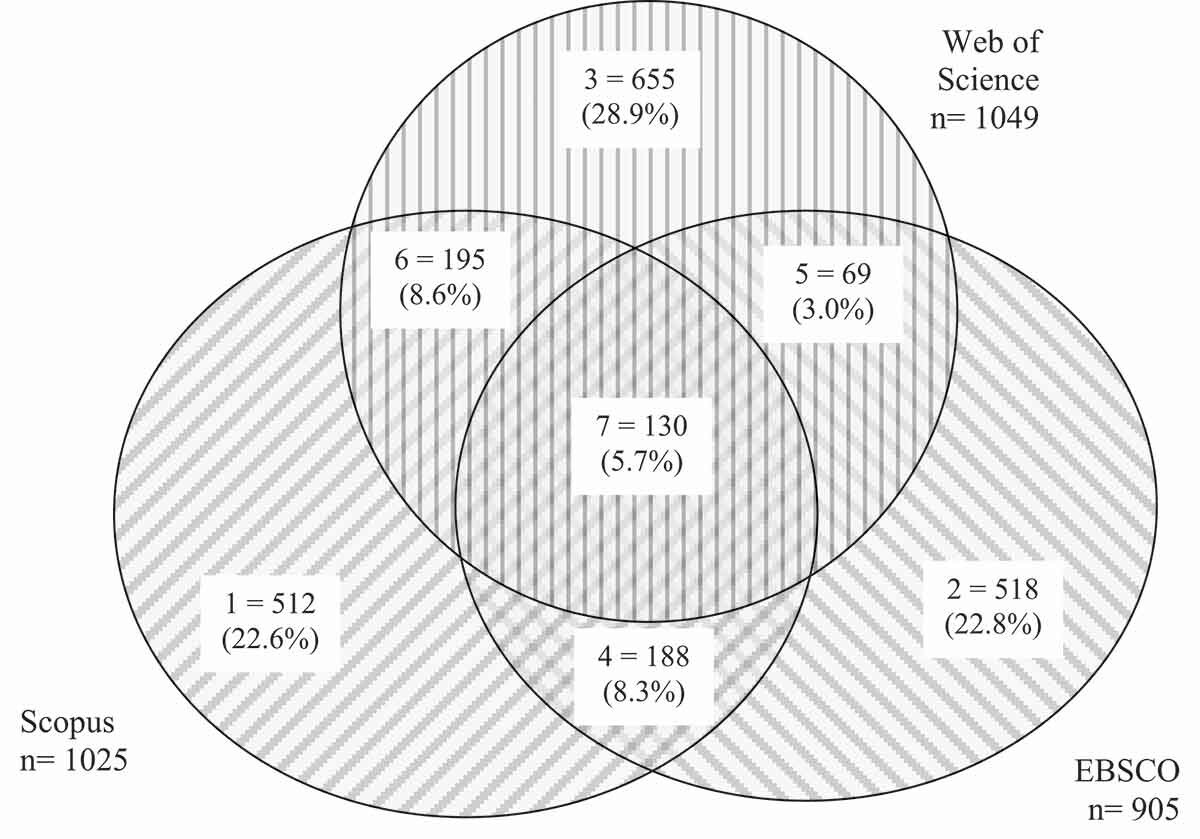
\includegraphics[width=.6\linewidth]{litSearchDBs.jpg}
        \caption{Distribution of searched articles across databases. \autocite{litSearch}}
        \label{fig:litSearch}
    \end{figure}
   
    \noindent 
    All searches performed will be on papers published during or after 2020, due to the 
    constantly evolving fields my project is based on. The search terms I will use to retrieve
    the data I will be studying are:

    \begin{itemize}
        \item Artifical Intelligence / AI 
        \begin{itemize}
            \item Ethics
            \begin{itemize}
                \item Bias
                \item Fairness
                \item Privacy
            \end{itemize}
        \end{itemize}
        \item Chatbots / Digital Assistants
        \item Generative AI
        \item Large Language Models / LLMs
        \begin{itemize}
            \item Fine tuning
        \end{itemize}
        \item Natural Language Processing / NLP
        \begin{itemize}
            \item Intent recognition
            \item Entity extraction
        \end{itemize}
        \item Deep learning
        \item User Experience / UX
        \begin{itemize}
            \item Design
        \end{itemize}
        \item Information retrieval
    \end{itemize}

    \noindent
    By using these specific terms that are directly relevant to the core themes of my project,
    I will be ensuring that I only retrieve literature that will be of crucial use in its 
    development.


    \chapter{Literature Review}

    \section{Themes}

    My project has many underlying themes, including:

    \begin{table}[H]
        \centering
        \begin{tabular}{|p{0.2\textwidth}|p{0.5\textwidth} | p{0.2\textwidth}|}
            \hline
            \cellcolor{blue!25}Theme & \cellcolor{blue!25}Description &
            \cellcolor{blue!25}Keywords \\

            \hline

            AI & A field of computing dedicated to allowing computers to simulate human
            learning by training them on large amounts of data so that they can recognise patterns to classify or 
            predict unknown data. AI can only be as good as the data it is trained upon, and can 
            develop biases if it is fed too much data of a certain type. & Generative AI, AI Ethics, AI Bias \\

            \hline

            Generative AI & AI dedicated to the generation of content rather than prediction or 
            classification. It is possible for generative AI to produce text, images and 
            more recently, even video and sound. & LLMs, Tokens, Embedding \\

            \hline
            Chatbot \newline Digital Assistant & Software that simulates a natural conversation between the 
            computer and end user. Many chatbots, including the one I intend to develop, utilise recent
            developments such as Generative AI and NLP to interpret and respond to user queries.
            \autocite{IBMChatbotDef}
            & User Experience, Conversational Design, Microsoft Bot Framework, Watson Assistant, ChatGPT \\

            \hline 

            LLM & Large Language Models are a type of AI dedicated to the recognition and generation of text.
            As suggested by their name, they are trained on enormous amounts of text data, which allows them 
            to have active conversations with users. There are many different LLMs, and as their size and 
            complexity increases, so too does the necessary processing power. &
            GPT4o, LLaMA, Gemini, Claude

            \\

            \hline

        \end{tabular}\label{tab:themes}
    \end{table}


    \section{Review of Literature}

    \subsection{Review}

    Check the template document because I'm not too sure if it's formatted this way.

    \subsection{Theory}

    Check the template document because I'm not too sure if it's formatted this way.
    
    \section{Summary}

    
    \begin{landscape}

    \chapter{Appendix}
    
    \begin{tcolorbox}[colback=red!5!white,colframe=red!75!black,title=Copied from proposal]
        This is still subject to change pending the feedback from my proposal.
    \end{tcolorbox}

    \section{Gantt Chart}



    \begin{figure}[H]
        \centering
        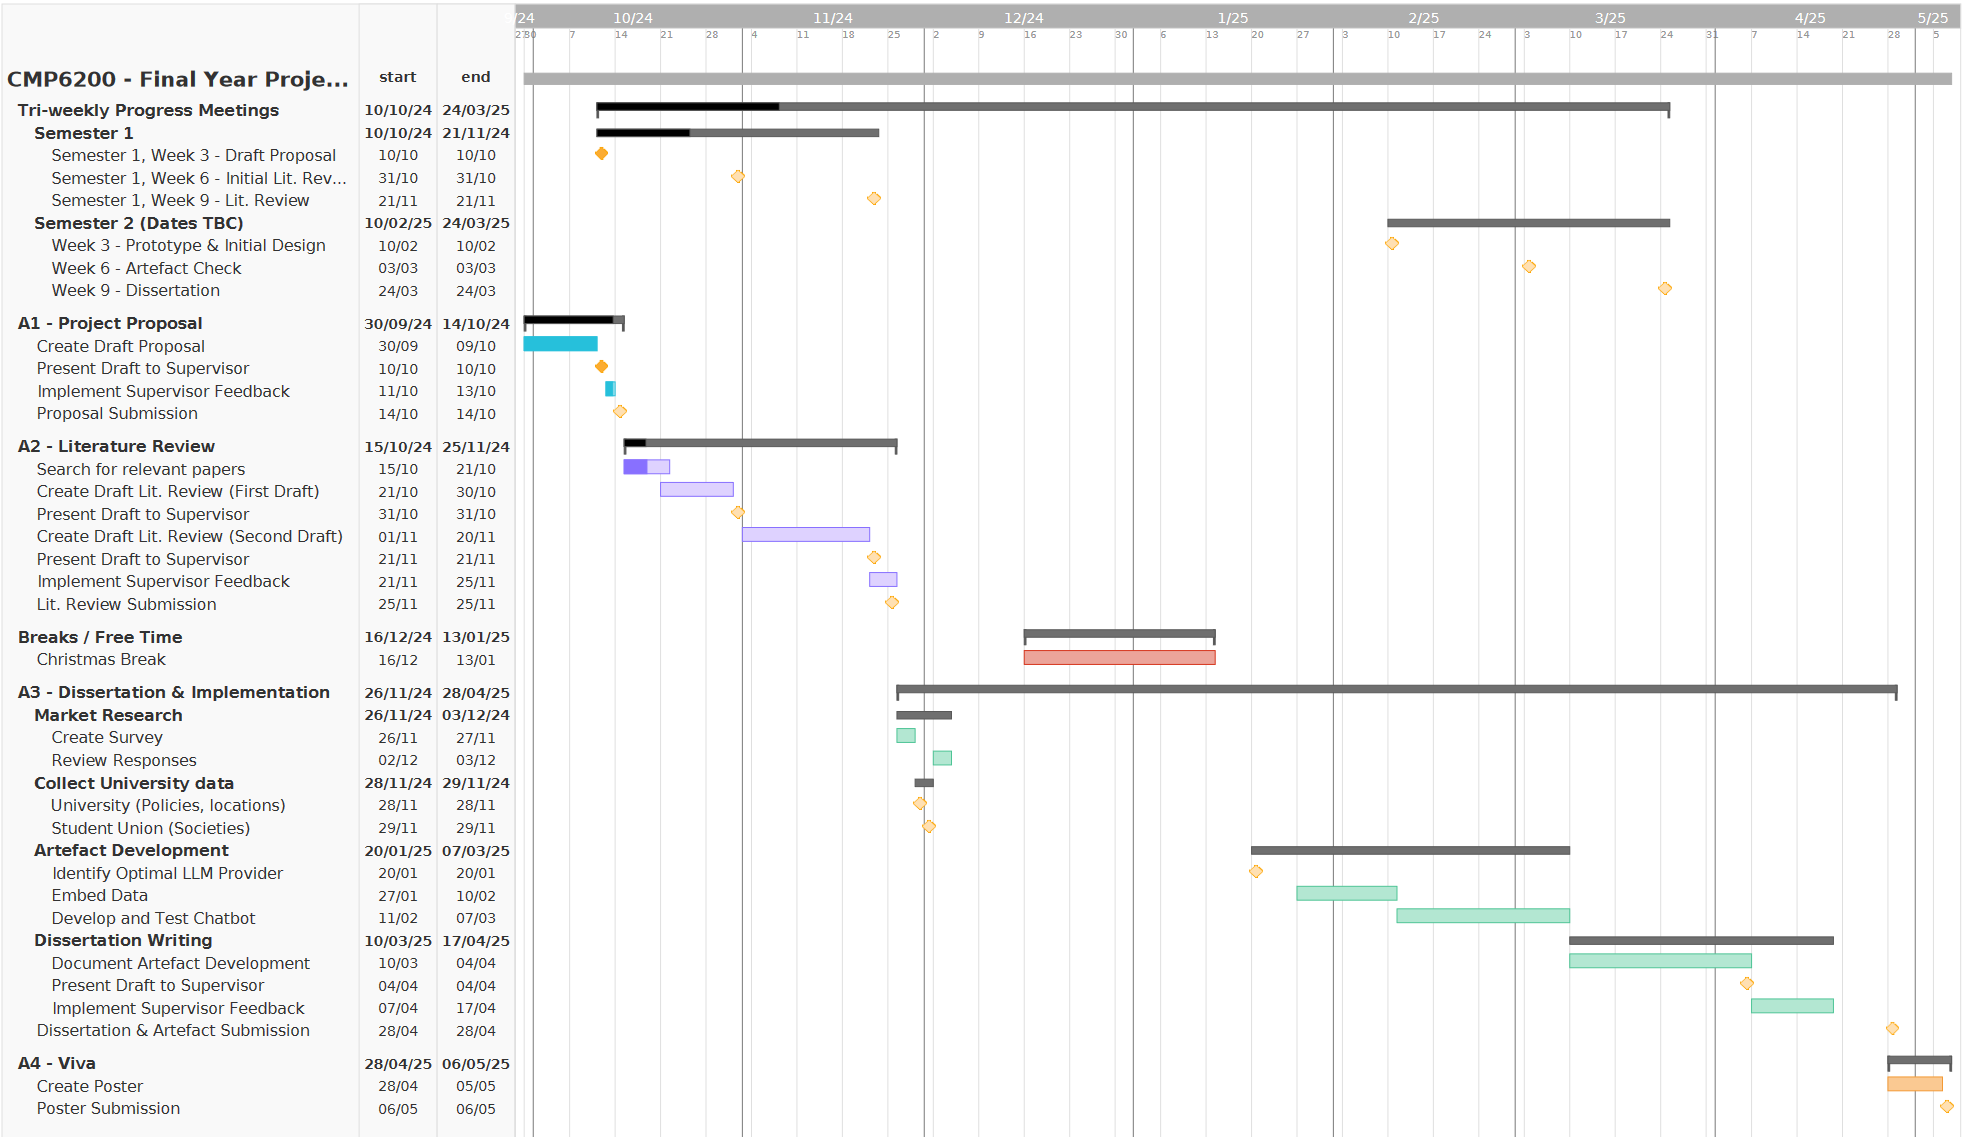
\includegraphics[width=.75\linewidth]{ProposalGantt.png}
        \caption{A conceptual Gantt chart of a development timeline.}
        \label{fig:gantt}
    \end{figure}

    \end{landscape}

    References and bibliographies aren't the same thing. Your references 
    are your directly cited sources, whereas your bibliography is everything you 
    consulted for information, even if you didn't directly cite it. \\

    \printbibliography[keyword={refs}, title = {References}]
    \addcontentsline{toc}{chapter}{References}

    % Invisible citing sources so that they get printed here
    \nocite{IBMAIDef}
    \nocite{ICOAIDef}
    \nocite{IBMGenAI}
    \nocite{MITGenAI}
    \nocite{CloudflareLLM}

    \printbibliography[keyword={bib}] % Will show an error until you cite an actual "bib" source.
    \addcontentsline{toc}{chapter}{Bibliography}

\end{document}